\documentclass[tikz,border=8pt]{standalone}
\usetikzlibrary{automata,positioning}
\begin{document}
% q0 = {0}
% q1 = {1, 3}
% q2 = {2}
% q3 = {2, 4}
% q4 = {2, 5}
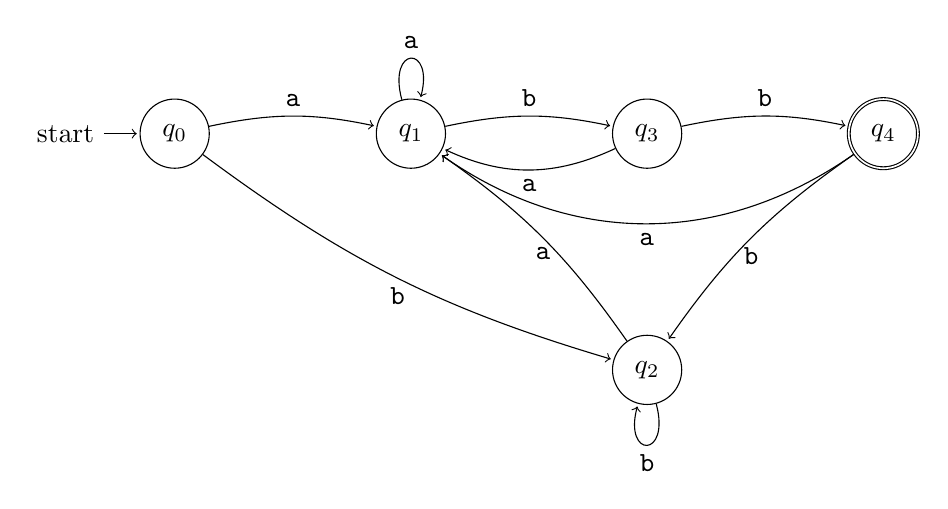
\begin{tikzpicture}[shorten >=1pt, node distance=3cm, on grid, auto]
  \node[state, initial] (q0) at (0,0) {$q_0$};
  \node[state] (q1) at (3,0) {$q_1$};
  \node[state] (q3) at (6,0) {$q_3$};
  \node[state, accepting] (q4) at (9,0) {$q_4$};
  \node[state] (q2) at (6,-3) {$q_2$};
  \path[->]
    (q0) edge [bend left=12] node[above] {\texttt{a}} (q1)
    (q0) edge [bend right=10] node[below] {\texttt{b}} (q2)
    (q1) edge [loop above] node[above] {\texttt{a}} (q1)
    (q1) edge [bend left=12] node[above] {\texttt{b}} (q3)
    (q2) edge [bend right=10] node[below] {\texttt{a}} (q1)
    (q2) edge [loop below] node[below] {\texttt{b}} (q2)
    (q3) edge [bend left=25] node[below] {\texttt{a}} (q1)
    (q3) edge [bend left=12] node[above] {\texttt{b}} (q4)
    (q4) edge [bend left=35] node[below] {\texttt{a}} (q1)
    (q4) edge [bend right=10] node[below] {\texttt{b}} (q2)
  ;
\end{tikzpicture}

\end{document}
